\documentclass[12pt]{beamer}
%\documentclass[20pt,handout]{beamer}
\usetheme{Darmstadt}
\usepackage{graphicx}
%\usepackage[german]{babel}
\usepackage{ngerman}
\usepackage[T1]{fontenc}
\usepackage[utf8]{inputenc}
\usepackage{tikz}
\setbeamertemplate{footline}[frame number]

\newcommand{\cc}[1]{\includegraphics[height=4mm]{img/#1.png}\hspace{1mm}}
\usepackage{ifthen}
\newcommand{\license}[2][]{\\#2\ifthenelse{\equal{#1}{}}{}{\\\scriptsize\url{#1}}}
\usepackage{textcomp}
\usepackage{hyperref}

\pgfdeclareimage[height=.6cm]{c3d2logo}{./img/c3d2.pdf}


\pgfdeclarelayer{foreground}
\pgfsetlayers{main,foreground}
\logo{\pgfputat{\pgfxy(-1,0)}{\pgfbox[center,base]{\pgfuseimage{c3d2logo}}}}


\title{Das sind doch nur Metadaten \\ Sicherheit im Netz}
\author{\small Stephan Thamm\\\large Chaos Computer Club Dresden}
\date{02.11.2016}

\begin{document}
\maketitle

\section{Einleitung}
\subsection{}

\begin{frame}
  \frametitle{Chaos Computer Club}
  \begin{figure}
    
\includegraphics[height=0.7\textheight]{img/fingerabdruck.jpg}
  \end{figure}
\end{frame}

\begin{frame}
    \frametitle{Chaos Computer Club}
    \begin{center}
	
\includegraphics[height=0.2\textheight]{img/chaosknoten.png}
    \end{center}	
    \begin{itemize}
      \item<1-> Verein wurde 1981 gegr"undet (\url{https://ccc.de})          
      \item<2-> Aktuell ca. 4500 Mitglieder
      \item<3-> Betreibt u.a. "Offentlichkeitsarbeit und Politikberatung      
      \item<4-> Lokale Erfahrungsaustauschkreise (Erfas) und Chaostreffs
    \end{itemize}
\end{frame}

\begin{frame}
  \frametitle{Chaos Computer Club Dresden}
  \begin{center}
    
\includegraphics[height=0.1\textheight]{img/c3d2_logo.png}
  \end{center}
  \begin{itemize}
    \item<1-> Chaos Computer Club Dresden (\url{https://c3d2.de})          
    \item<2-> Datenspuren (\url{https://datenspuren.de})
    \item<3-> Radio und Podcasts (\url{https://c3d2.de/radio.html})
    \item<4-> Chaos macht Schule (\url{https://c3d2.de/schule.html})
  \end{itemize}
\end{frame}

\section{Vorratsdatenspeicherung}
\subsection{}

\begin{frame}
  \frametitle{Metadaten}
  \only<2>{
    \begin{center}
      \fbox{
        
\includegraphics[height=0.7\textheight]{img/psb.png}
      }
    \end{center}
  }
  \only<3>{
    \begin{center}
      \large Metadaten oder Metainformationen sind Daten, die Informationen über Merkmale anderer Daten enthalten, aber nicht diese Daten selbst.
    \end{center}
  }
\end{frame}

\begin{frame}
  \frametitle{Vorratsdatenspeicherung}
  \begin{itemize}
    \item<2-> Standortdaten der Teilnehmer aller Mobiltelefonate bei Beginn des Telefonats, zu speichern für 4 Wochen
    \item<3-> Standortdaten bei Beginn einer mobilen Internetnutzung, zu speichern für 4 Wochen
    \item<4-> Rufnummern, Zeit und Dauer aller Telefonate, zu speichern für 10 Wochen
    \item<5-> Rufnummern, Sende- und Empfangszeit aller SMS-Nachrichten, zu speichern für 10 Wochen
    \item<6-> zugewiesene IP-Adressen aller Internetnutzer sowie Zeit und Dauer der Internetnutzung, zu speichern für 10 Wochen
  \end{itemize}
\end{frame}

\begin{frame}
  \frametitle{Bewegungsdaten}
  \pause
  \begin{center}
    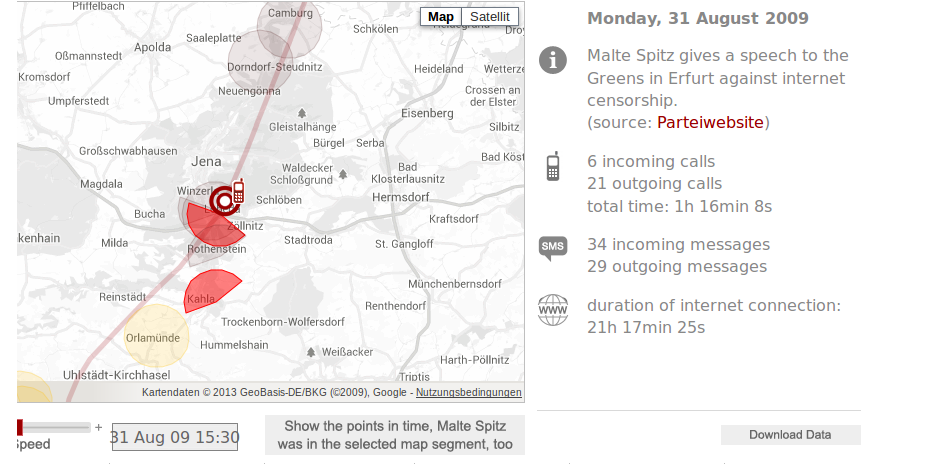
\includegraphics[height=0.7\textheight]{img/maltespitz.png}
  \end{center}
\end{frame}

\begin{frame}
  \frametitle{Verbindungsdaten}
  \begin{center}
    \only<1>{
      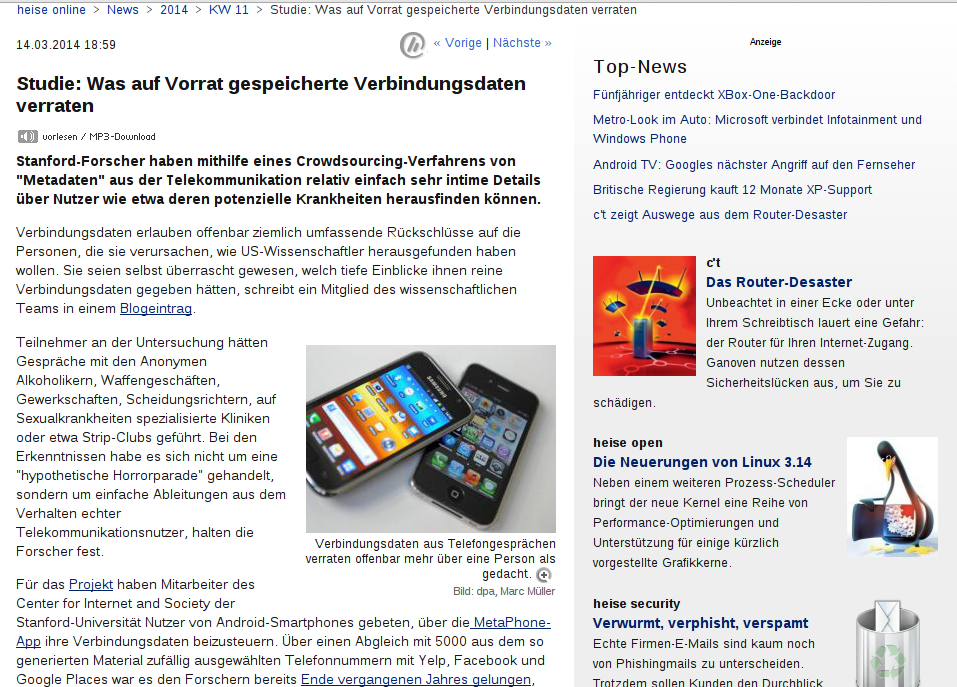
\includegraphics[height=0.7\textheight]{img/metadaten_studie.png}
    }
    \only<2>{
      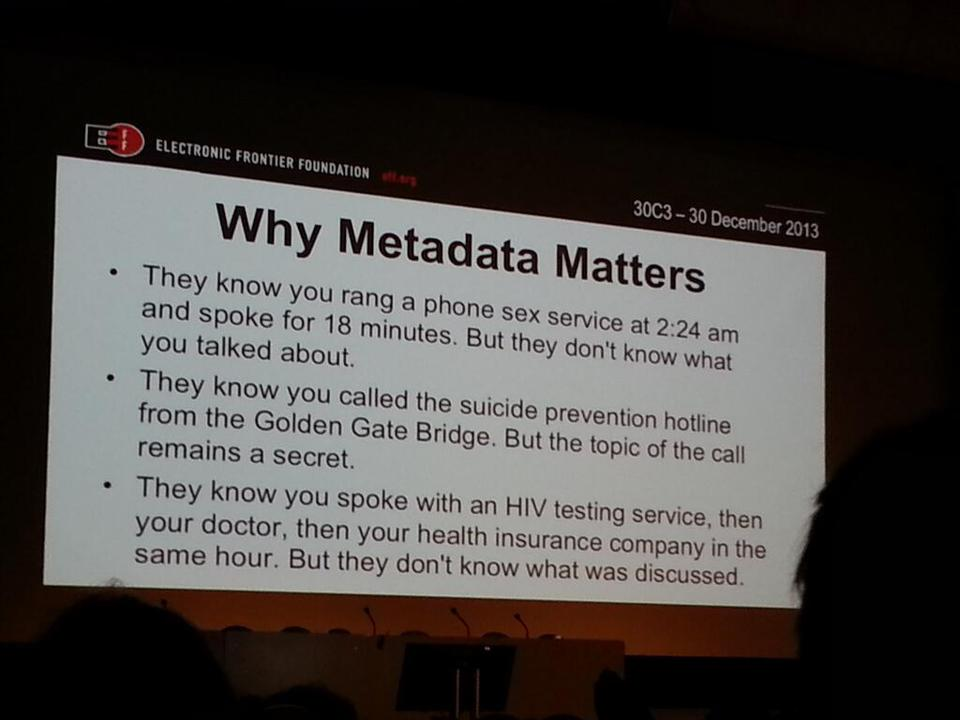
\includegraphics[height=0.7\textheight]{img/metadata-matters.jpg}
    }
  \end{center}
\end{frame}

\section{Geheimdienste}
\subsection{}

\begin{frame}
    \frametitle{Bundespräsident Gauck zur NSA-Überwachung}
    \begin{center}
      ``Wir wissen z.B., dass es nicht so ist, wie bei der Stasi und dem KGB, dass es dicke Aktenbände gibt, wo unsere Gesprächsinhalte alle aufgeschrieben und schön abgeheftet sind. Das ist es nicht.''
      (Gauck, 30.06.2013 im ZDF-Sommerinterview)
    \end{center}
\end{frame}

\begin{frame}
    \frametitle{Stasi vs. NSA}
    \begin{center}
	\only<1>{
		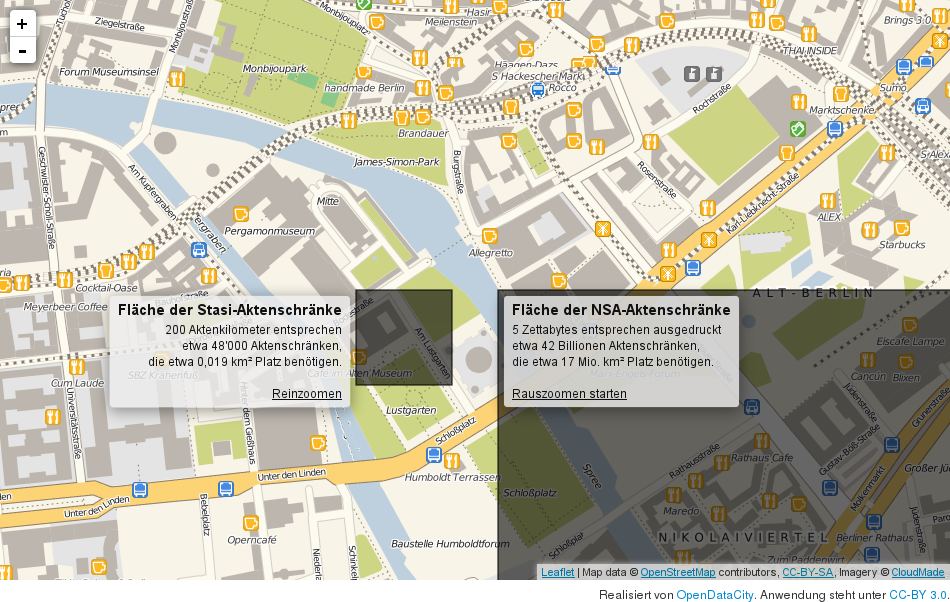
\includegraphics[height=0.7\textheight]{img/akten1.png}
	}
	\only<2>{
		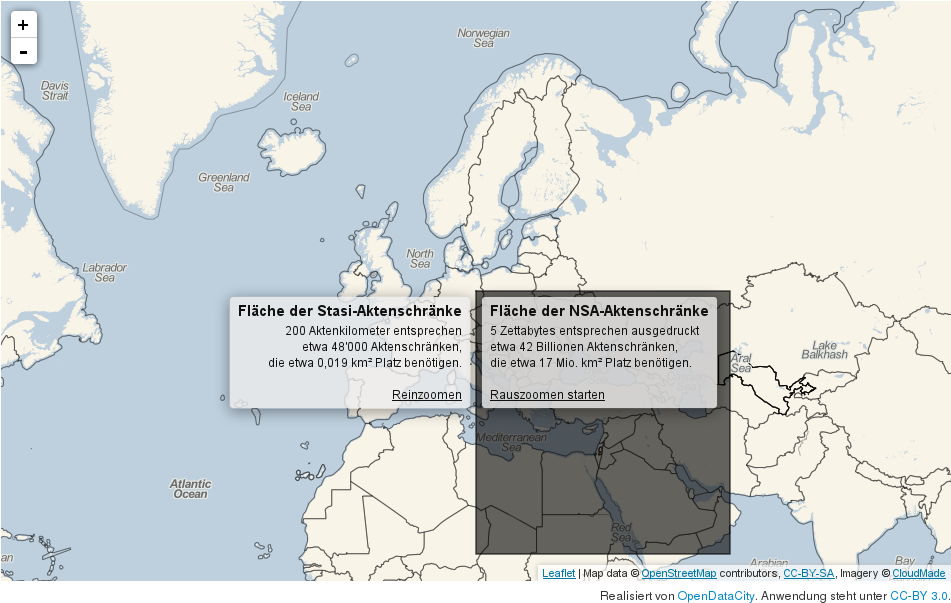
\includegraphics[height=0.7\textheight]{img/akten2.png}
	}
    \end{center}
\end{frame}

\begin{frame}
    \frametitle{NSA-Skandal}
    \begin{center}
	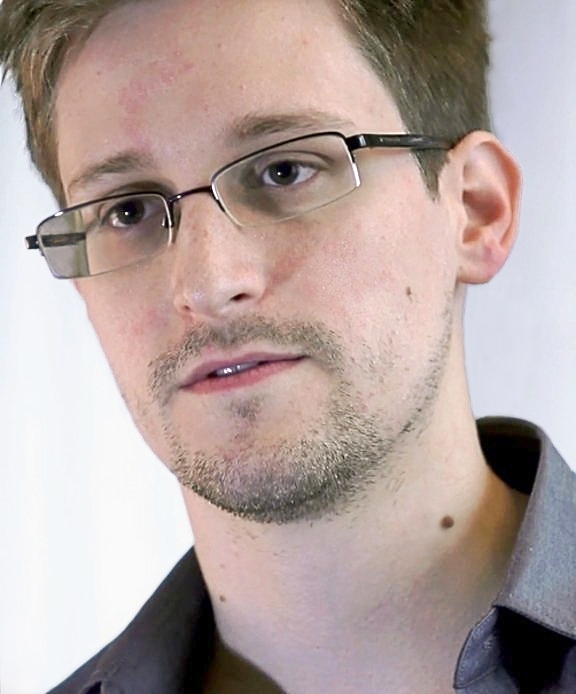
\includegraphics[height=0.7\textheight]{img/snowden.jpg}
    \end{center}	
\end{frame}

\begin{frame}
  \frametitle{Internet}
  \begin{center}
    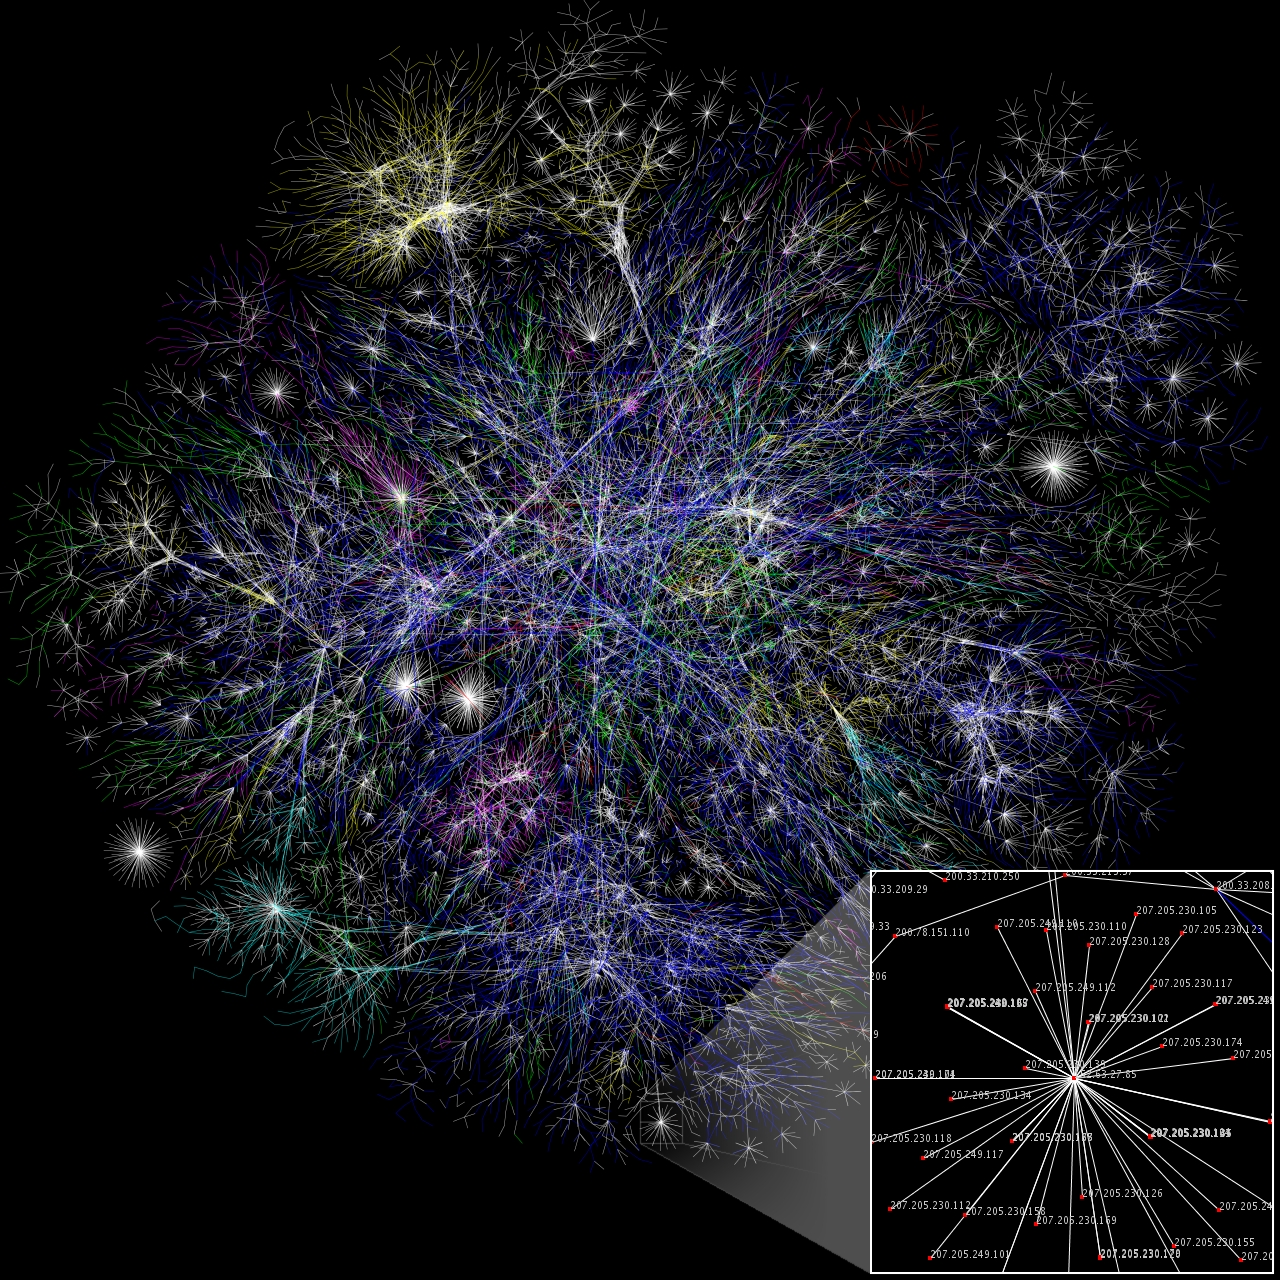
\includegraphics[height=0.7\textheight]{img/internet.jpg}
  \end{center}
\end{frame}

\begin{frame}
    \frametitle{Tempora}
    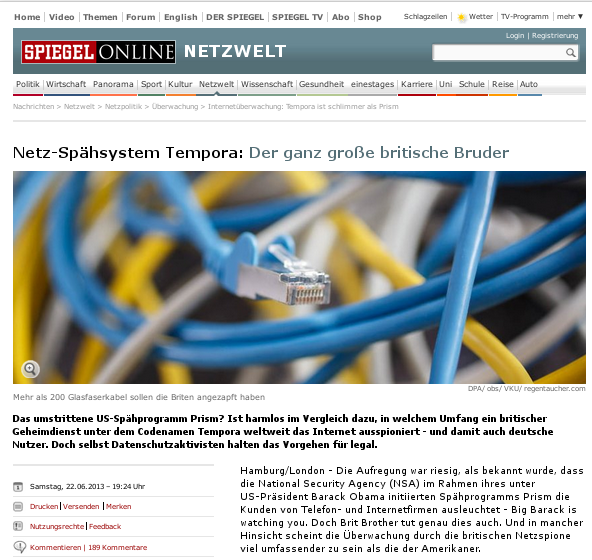
\includegraphics[height=0.7\textheight]{img/spiegel-tempora.png}
\end{frame}

\begin{frame}
    \frametitle{Prism}
    \begin{center}
	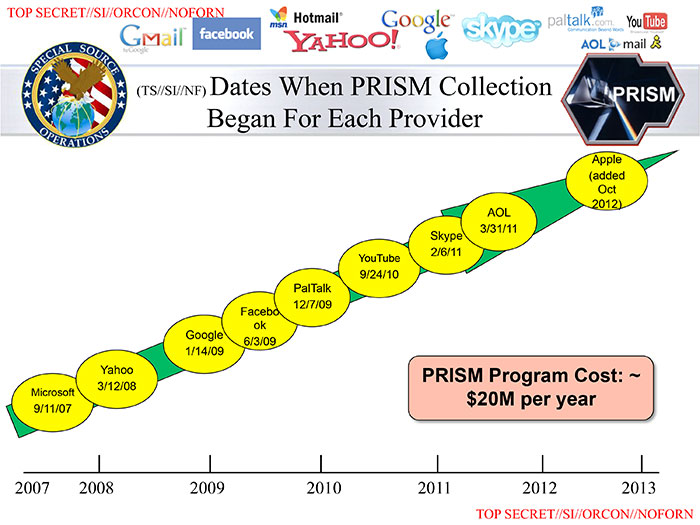
\includegraphics[height=0.7\textheight]{img/prism.jpg}
    \end{center}
\end{frame}

\begin{frame}
  \frametitle{Verhaltensänderung}
  \begin{center}
    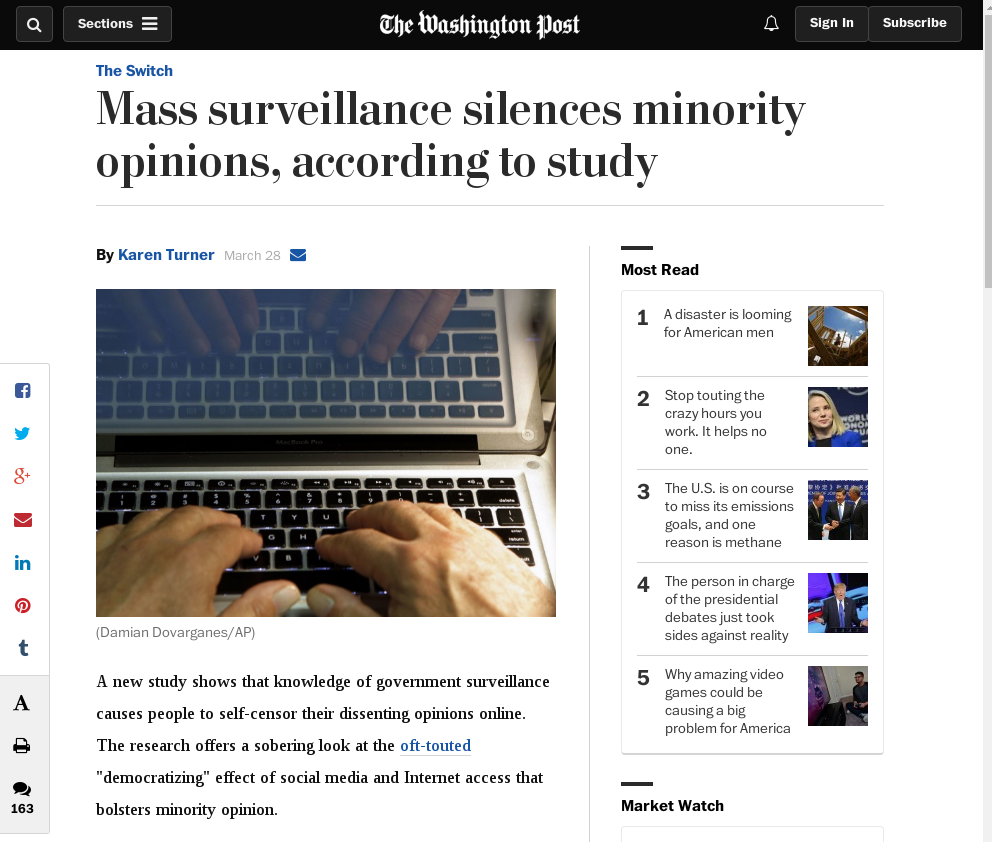
\includegraphics[height=0.7\textheight]{img/verhalten.png}
  \end{center}
\end{frame}

\begin{frame}
  \frametitle{Was tun die USA mit Metadaten?}
  \pause
  \begin{center}
    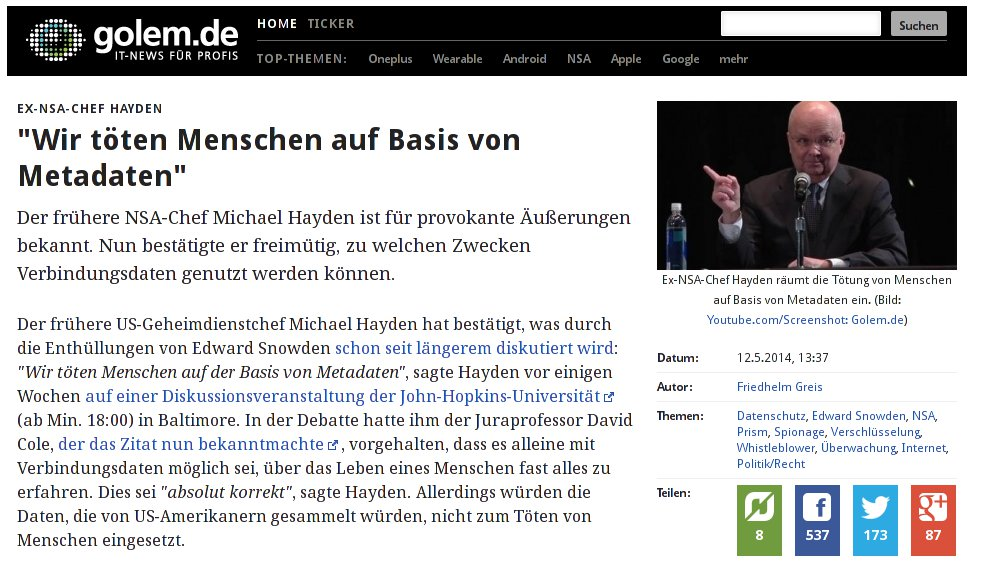
\includegraphics[height=0.7\textheight]{img/wekillpeople.jpg}
  \end{center}
\end{frame}

\begin{frame}
  \frametitle{Skynet}
  \begin{center}
    \only<2>{
      
\includegraphics[height=0.7\textheight]{img/terminator.jpg}
    }
    \only<3>{
      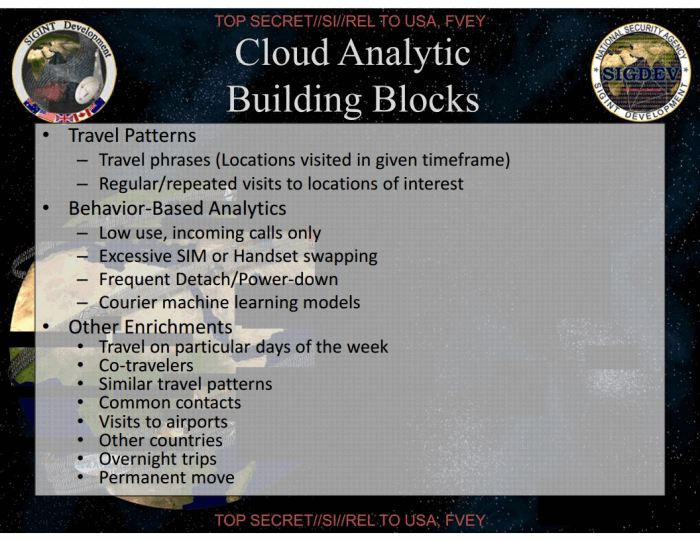
\includegraphics[height=0.7\textheight]{img/skynet.png}
    }
    \only<4>{
      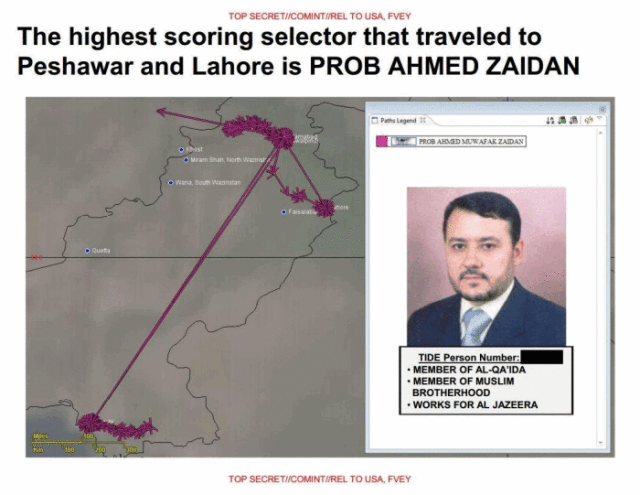
\includegraphics[height=0.7\textheight]{img/skynet2.png}
    }
  \end{center}
\end{frame}

\section{Wirtschaft}
\subsection{}

\begin{frame}
  \frametitle{Firmen}

  \begin{itemize}
    \item Womit verdienen folgende Firmen ihr Geld?
      \begin{itemize}
        \item<2-> Karstadt
        \item<3-> Amazon
        \item<4-> Ebay
        \item<5-> Facebook
      \end{itemize}
  \end{itemize}
\end{frame}

\begin{frame}
  \frametitle{Gesch"aftsmodelle}
  \begin{figure}
    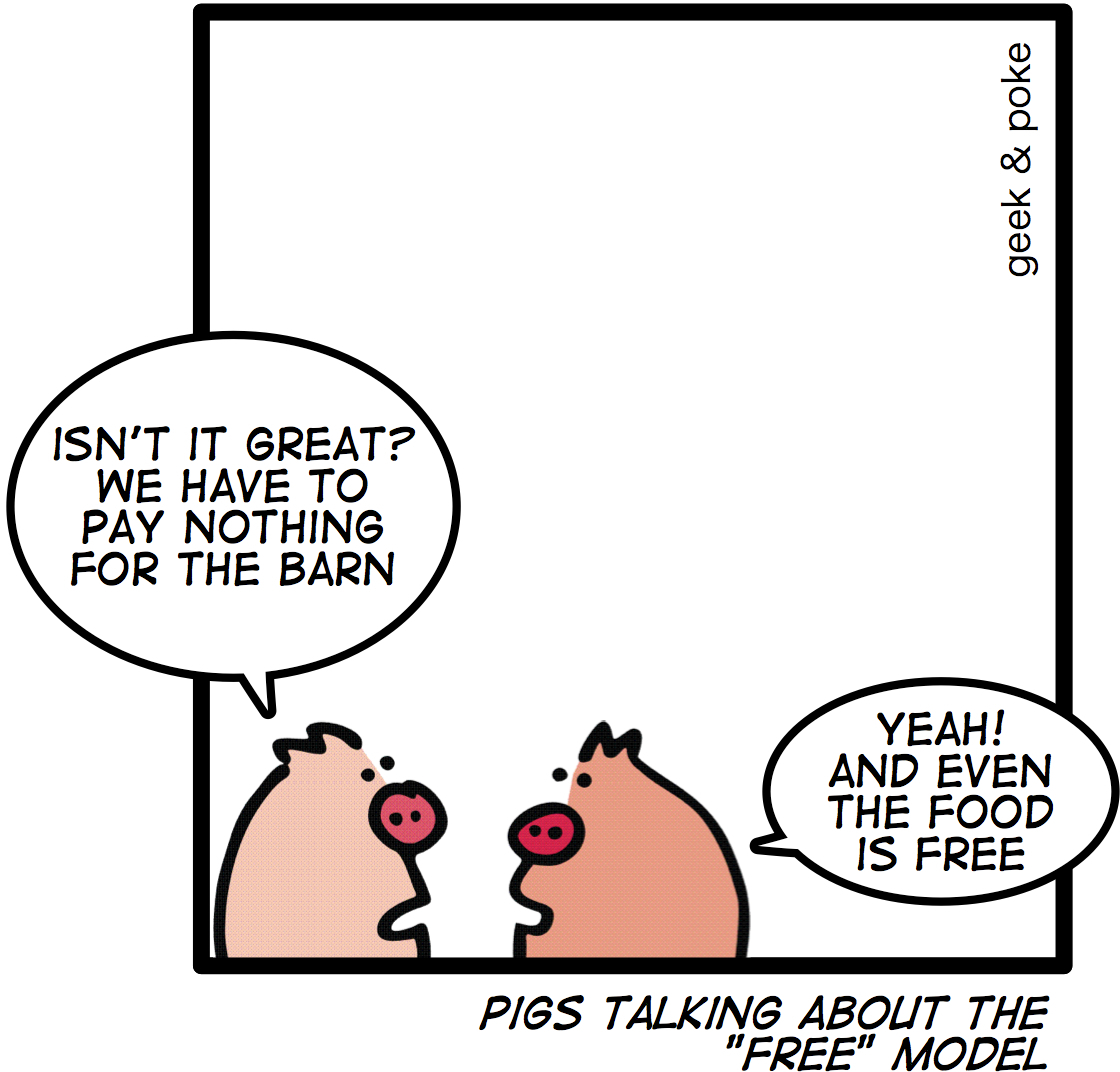
\includegraphics[height=0.7\textheight]{img/business_pigs.jpg}
  \end{figure}
\end{frame}

\begin{frame}
  \frametitle{Soziale Netzwerke}

  \begin{itemize}
    \item Was haben soziale Netzwerke von ihren Nutzen?\\(am Bsp. von Facebook)
      \begin{itemize}
        \item<2-> 82\% Einnahmen aus Werbung
        \item<3-> 30\% Anteil an "`Facebook-Einkäufen"'
        \item<4-> durchschnittlich 1€/Profil
        \item<5-> "`Poweruser"'-Profile deutlich mehr
        \item<6-> => Mehr Werbegewinn durch personalisierte Werbung
	\item<7-> Q2 2014 791 Mio Dollar Gewinn
      \end{itemize}
  \end{itemize}
\end{frame}

\begin{frame}
  \frametitle{Telefonica}
  \pause
  \begin{center}
    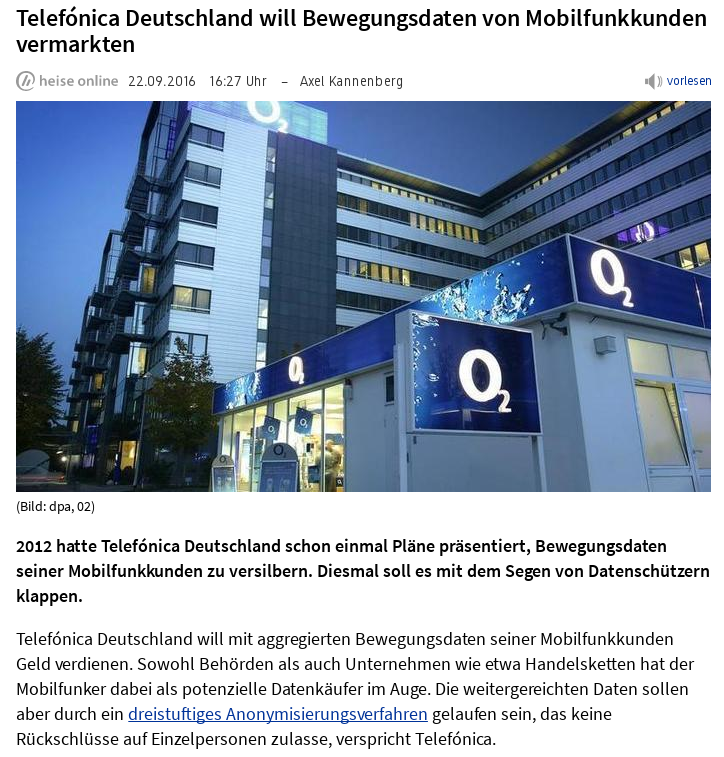
\includegraphics[height=0.7\textheight]{img/telefonica.png}
  \end{center}
\end{frame}

\begin{frame}
  \frametitle{Google}
  \begin{center}
    
\includegraphics[height=0.4\textheight]{img/google.jpg}
  \end{center}
\end{frame}

\begin{frame}
  \frametitle{Werbenetzwerke}
  \begin{center}
    \only<2>{
      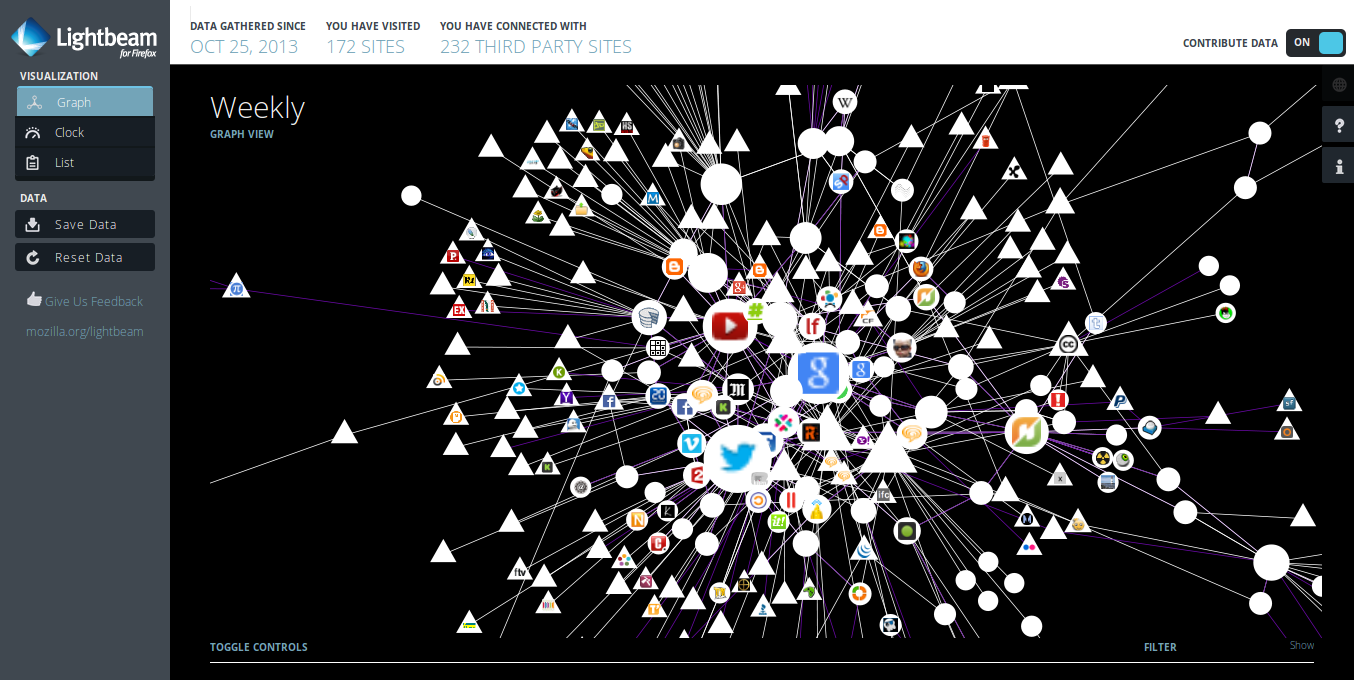
\includegraphics[height=0.7\textheight]{img/lightbeam.png}
    }
    \only<3>{
      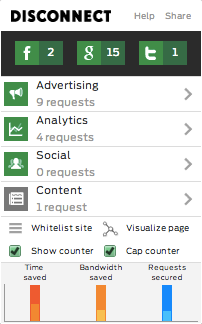
\includegraphics[height=0.7\textheight]{img/disconnect.png}
    }
  \end{center}
\end{frame}

\begin{frame}
  \frametitle{Gezielte Werbung}
  \pause
  \begin{center}
    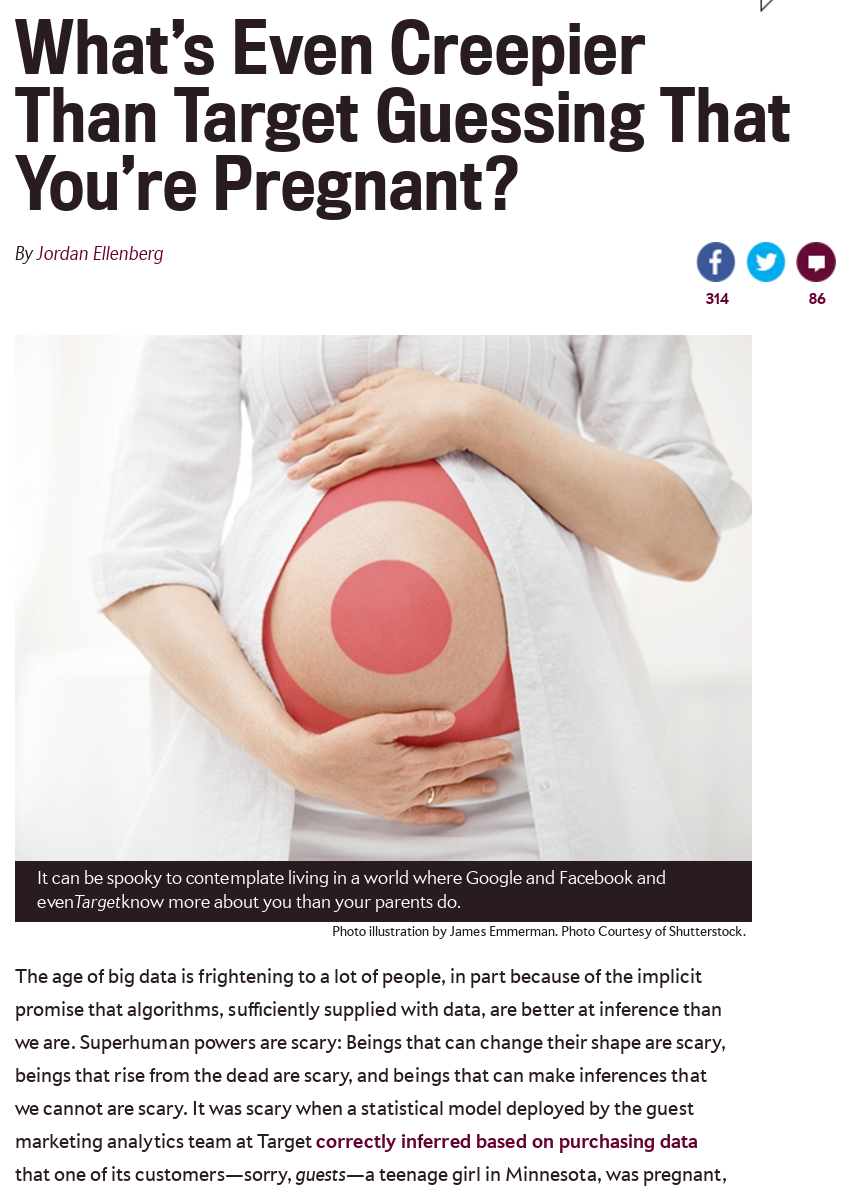
\includegraphics[height=0.8\textheight]{img/pregnant.png}
  \end{center}
\end{frame}

\begin{frame}
	\frametitle{Datenanalyse - Zeit}
  \begin{center}
    \only<2>{
      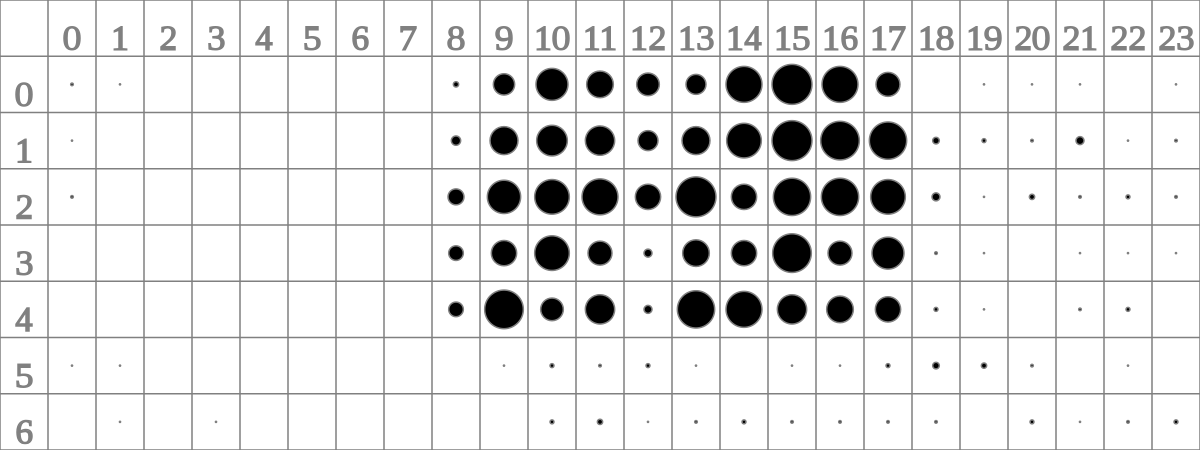
\includegraphics[height=0.4\textheight]{img/punch_1.png}
    }
    \only<3>{
      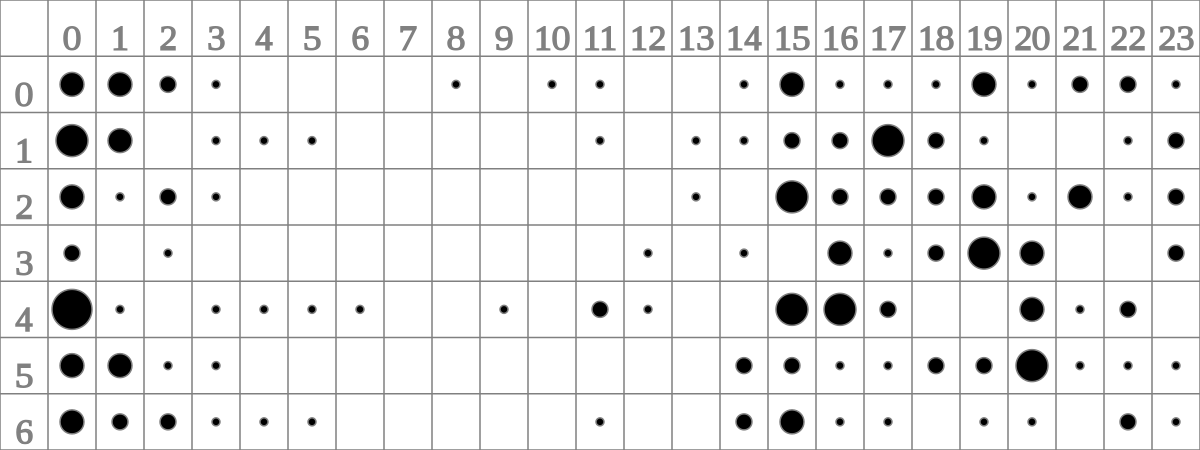
\includegraphics[height=0.4\textheight]{img/punch_2.png}
    }
    \only<4>{
      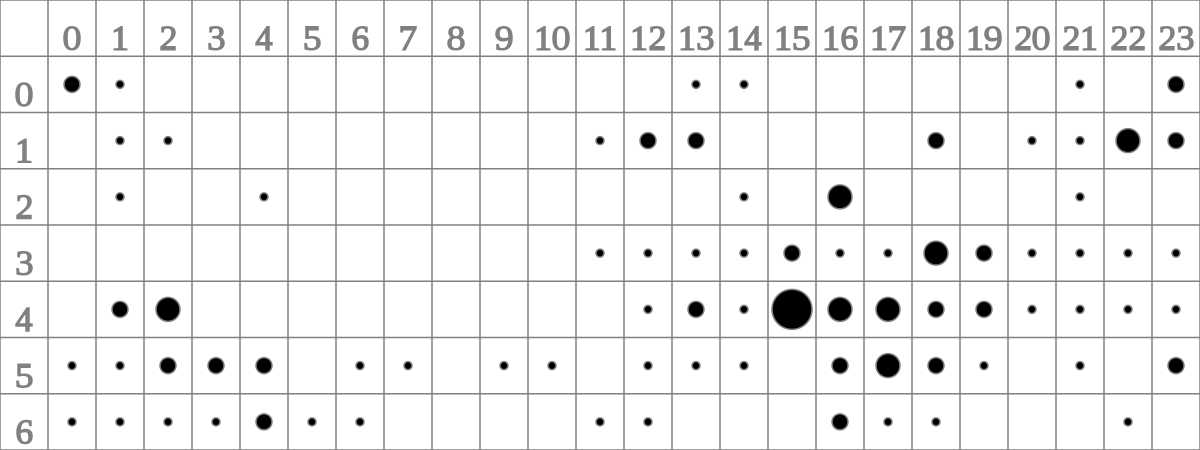
\includegraphics[height=0.4\textheight]{img/punch_3.png}
    }
  \end{center}
\end{frame}

\section{Gegenmaßnahmen}
\subsection{}

\begin{frame}
  \frametitle{SSL}
  \begin{center}
    \only<2>{
      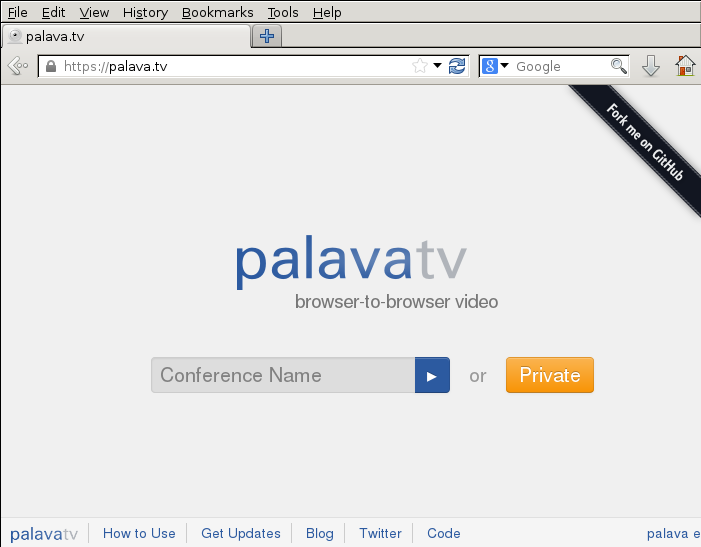
\includegraphics[height=0.7\textheight]{img/ssl_verified.png}
    }
    \only<3>{
      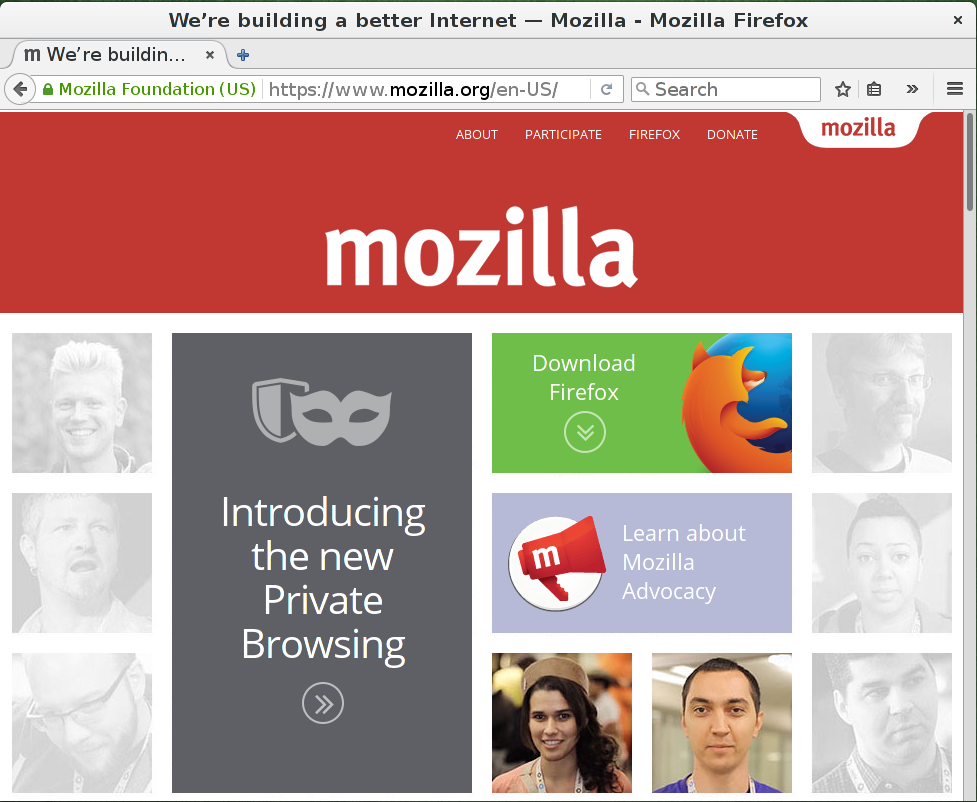
\includegraphics[height=0.7\textheight]{img/ssl_special.png}
    }
    \only<4>{
      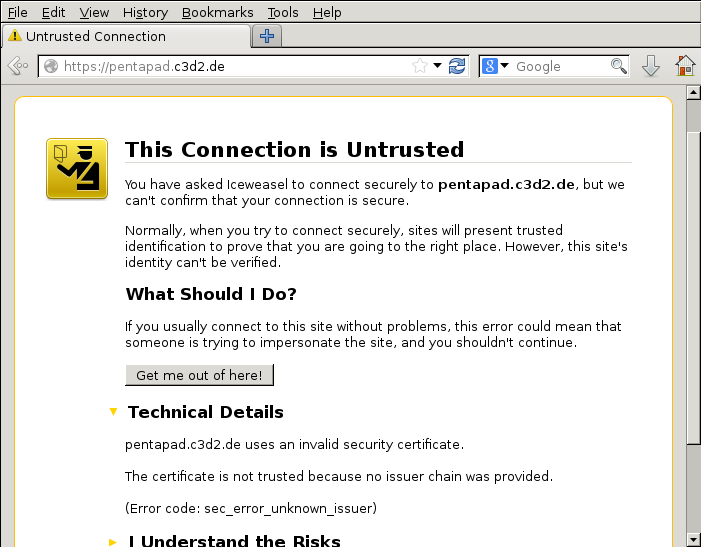
\includegraphics[height=0.7\textheight]{img/ssl_unverified.png}
    }
  \end{center}
\end{frame}

\begin{frame}
  \frametitle{TOR}
  \begin{center}
    \only<2>{
      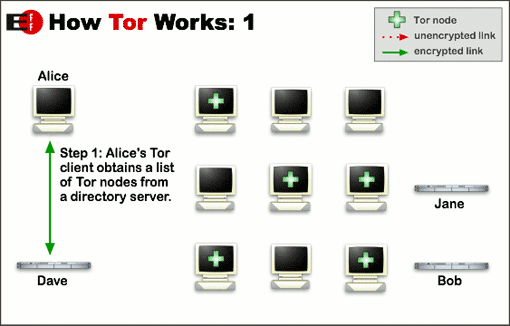
\includegraphics[height=0.7\textheight]{img/tor1.png}
    }
    \only<3>{
      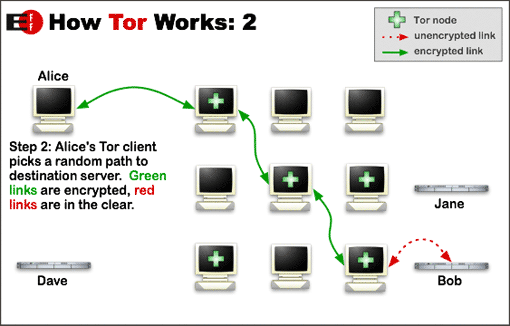
\includegraphics[height=0.7\textheight]{img/tor2.png}
    }
    \only<4>{
      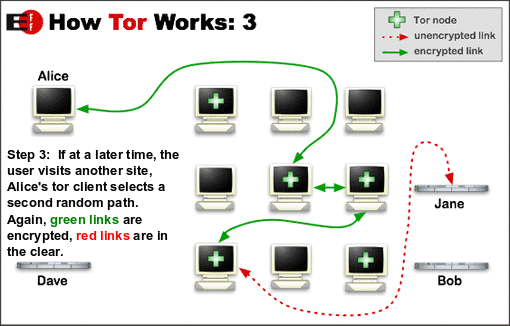
\includegraphics[height=0.7\textheight]{img/tor3.png}
    }
  \end{center}
\end{frame}

\begin{frame}
  \frametitle{Alternative Dienste und Software}
  \begin{center}
	\large{Alternative Dienste und Software}
  \end{center}
\end{frame}

\begin{frame}
  \frametitle{Datensparsamkeit}
  \begin{center}
	\large{Datensparsamkeit}
  \end{center}
\end{frame}

\begin{frame}
  \frametitle{Passwortsicherheit}
  \begin{center}
	\large{Passwortsicherheit}
  \end{center}
\end{frame}

\section{Fazit}
\subsection{}

\begin{frame}
  \frametitle{Fazit}
  \begin{itemize}
    \item<2-> immer mehr Daten
    \item<3-> hohes Missbrauchspotential
    \item<4-> Metadaten schwer technisch vermeidbar
    \item<5-> Problembewusstsein
    \item<6-> Verantwortungsvoller Umgang
  \end{itemize}
\end{frame}

\end{document}
